\section{Введение}
\label{sec:intro}

Обработка данных является важной задачей для крупных компаний. Такого рода задача решается с помощью написания процессингов данных. Код с помощью базы данных описывает некоторый граф или, иначе, pipeline. По нему данные перемещаются из одной системы в другую, попутно происходит их обогащение или, наоборот, фильтрация.

Существует два вида обработки больших объемов данных: batch и streaming.

Batch подразумевает обработку больших массивов данных, предварительно сохраненных в некотором хранилище, то есть все данные готовы к процессингу перед запуском pipeline-а. В таком типе обработки важна пропускная способность (throughput), инфраструктура должна справляться с тяжелыми вычислениями. Примером такого процессинга может быть построение выжимки из поисковый сессий пользователя за день.

Streaming предполагает, что мы обрабатываем данные, которые поступают к нам некоторыми порциями (micro-batch), причем они не известны в полном объеме на момент запуска pipeline-а. В таком роде pipeline-ов часто оказывается важно максимальное время, затраченное на обработку порции данных. Примером такого процессинга может являться некоторая агрегация самой актуальной информации о поисковых запросах человека.

Помимо прочего два рассмотренных подхода объединяет то, что логика процессинга данных не зависит от способа обработки. Действительно, в случае batch процессингов данные могут быть обогащены более сложно вычислимыми статистиками. Однако с точки зрения, например, библиотеки для выражения логики на некотором языке программирования логика может быть представлена композицией функций многих входов и выходов. Более точная классификация такова: произвольные функции, модифицирующие, фильтрующие или мультиплицирующие данные (Map) и функции группировки (Reduce) по выделенному из данных ключу [ссылка].

Благодаря тому, что логика выражается с помощью набора примитивов, есть возможность написать библиотеку, которая предоставит общее API для написания различных процессингов. Такая библиотека под названием “Roren” была написана в Яндексе [ссылка].

\newpage
\subsection{Постановка задачи}

Инструмент должен решать задачу тестирования распределенной системы, внутри которой исполняется код студента.

Распределенную систему мы представим в виде набора узлов, объединенных в общую сеть. Узлы могут коммуницировать друг с другом только с помощью отправки сообщений.

Сеть мы считаем асинхронной и недетерминированной – она может произвольно задерживать и переупорядочивать отправляемые узлами сообщения. Если система будет корректно работать в асинхронной сети, то и в реальной, частично синхронной сети тоже.

Внутри узла исполняются недетерминированные программы. Также узлы могут отказывать, то есть перезагружаться в произвольные моменты и/или навсегда отключаться.

Мы считаем, что набор узлов системы реализует некоторый распределенный сервис, с которым клиенты взаимодействуют через протокол RPC. 

Клиенты тоже являются узлами сети. 

Они посылают системе запросы и получают ответы, в результате возникает конкурентная история, состоящая из отрезков запросов (рис.~\ref{fig:history_example}). Свойства системы формулируются как утверждения про допустимые истории, которые может порождать система.

\begin{figure}[h]
    \centering
    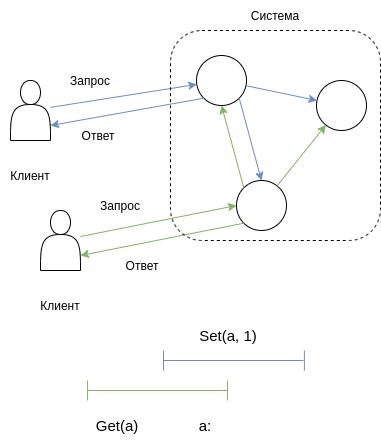
\includegraphics[width=0.5\textwidth]{img/task.png}
    \caption{Пример истории запросов}
    \label{fig:history_example}
\end{figure}

В данной работе нас прежде всего интересует задача репликации, так что распределенный сервис  представляет собой хранилище данных с операциями Set и Get, а свойство, которое мы ожидаем от системы – модель согласованности \cite{consistency}, в первую очередь – линеаризуемость \cite{linearizability}.

Наконец, сформулируем задачу – по реализации узлов системы проверить выполнение заявленных свойств независимо от поведения сети между узлами, часов и т.д.


\newpage
\subsection{Цель работы}

Цель работы состоит в реализации части библиотеки Roren, отвечающей за перевод и выполнение pipeline-ов поверх YT. Компонент должен позволять запускать произвольные графы обработки данных, выражаемые операциями Map/Reduce.

Получившаяся реализация в сравнении с текущей должна:
\begin{itemize}
    \item Переводить pipeline-ы в графы с меньшим количеством YT операций
    \item Иметь расширяемый на более сложные YT операции алгоритм трансляции
\end{itemize}


\newpage
\subsection{План работы}

Во второй главе мы рассмотрим дизайн библиотеки Roren: от API pipeline-ов до запуска YT операций.

В третьей главе рассмотрим реализацию компонента, производящего трансляцию. Мы изложим этапы перевода roren графа в граф YT операций, алгоритм трансляции, и детально остановимся на компоненте оптимизатора.

В четвертой главе посмотрим на примеры графов и их трансляций, обсудим тестирование.

В последней главе мы поговорим о результатах работы и обсудим пути развития компонента.

